\documentclass[varwidth=true, border=2pt]{standalone}
\usepackage{tikz}
\begin{document}

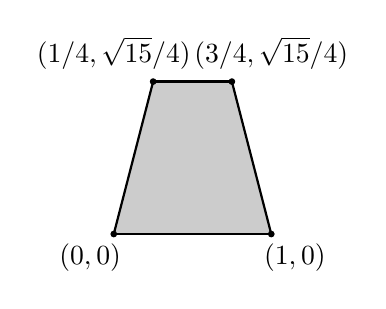
\begin{tikzpicture}[line join=bevel,z=-5.5]
    \coordinate (0) at (0,0);
    \coordinate (1) at (2,0);
    \coordinate (2) at (1.5,1.936);
    \coordinate (3) at (0.5,1.936);
    \node at (-0.3, -0.3) {$(0,0)$};
    \node at (2.3, -0.3) {$(1,0)$};
    \node at (2, 2.3) {($3/4,\sqrt{15}/4$)};
    \node at (0, 2.3) {($1/4,\sqrt{15}/4$)};

%   \draw  -- (B1) -- cycle;
%\draw (A4) -- (A1) -- (B1) -- cycle;
    \fill[black!20!white] (0) -- (1) -- (2) -- (3) -- cycle;
    \draw[fill=black] (0) circle (1pt);
    \draw[fill=black] (1) circle (1pt);
    \draw[fill=black] (2) circle (1pt);
    \draw[fill=black] (3) circle (1pt);
    \draw[thick] (0) -- (1);
    \draw[thick] (1) -- (2);
    \draw[thick] (2) -- (3);
    \draw[thick] (3) -- (0);
\end{tikzpicture}

\end{document}